\documentclass{specification}
\usepackage[backend=bibtex]{biblatex}
\usepackage{dsfont}
\usepackage{graphicx}
\usepackage{epstopdf}
\usepackage{booktabs}
\usepackage{csquotes}
\bibliography{bibliography}


\title{Automated Protein Function Description for Novel Class Discovery}
\author{Meet Barot, Vladimir Gligorijevic, Kyunghyun Cho, Richard Bonneau}

\begin{document}

\maketitle

\section{Abstract}
Knowledge of protein function is necessary for understanding biological systems, but functional characterization is far outpaced by the discovery of new sequences from high-throughput sequencing technologies.
Beyond the difficulty of assigning newly sequenced proteins to known functions, a more challenging issue is discovering novel protein functions.
Protein function prediction, as it is usually framed in the case of Gene Ontology term prediction, is a multilabel problem with a hierarchical label space.
However, this framing is limiting. It does not provide guiding principles for discovering completely novel functions.
Clustering-based approaches are not able to give much information about the new functional categories that they predict; they can only predict that a protein may belong to a category that has not been studied.
In this work we propose a neural machine translation model in order to generate descriptions of protein functions in natural language.
The model takes as input a set of sequences, and assigns a probability to any description paired with those sequences.
We define three metrics that can be computed using our model's probabilities assignment of known functional descriptions to input sequence sets.
We provide quantitative results of our model in the zero-shot classification setting, scoring sequence sets with functional descriptions that the model has not seen before, as well as generated function descriptions for qualitative evaluation.

\begin{figure}
    \centering
    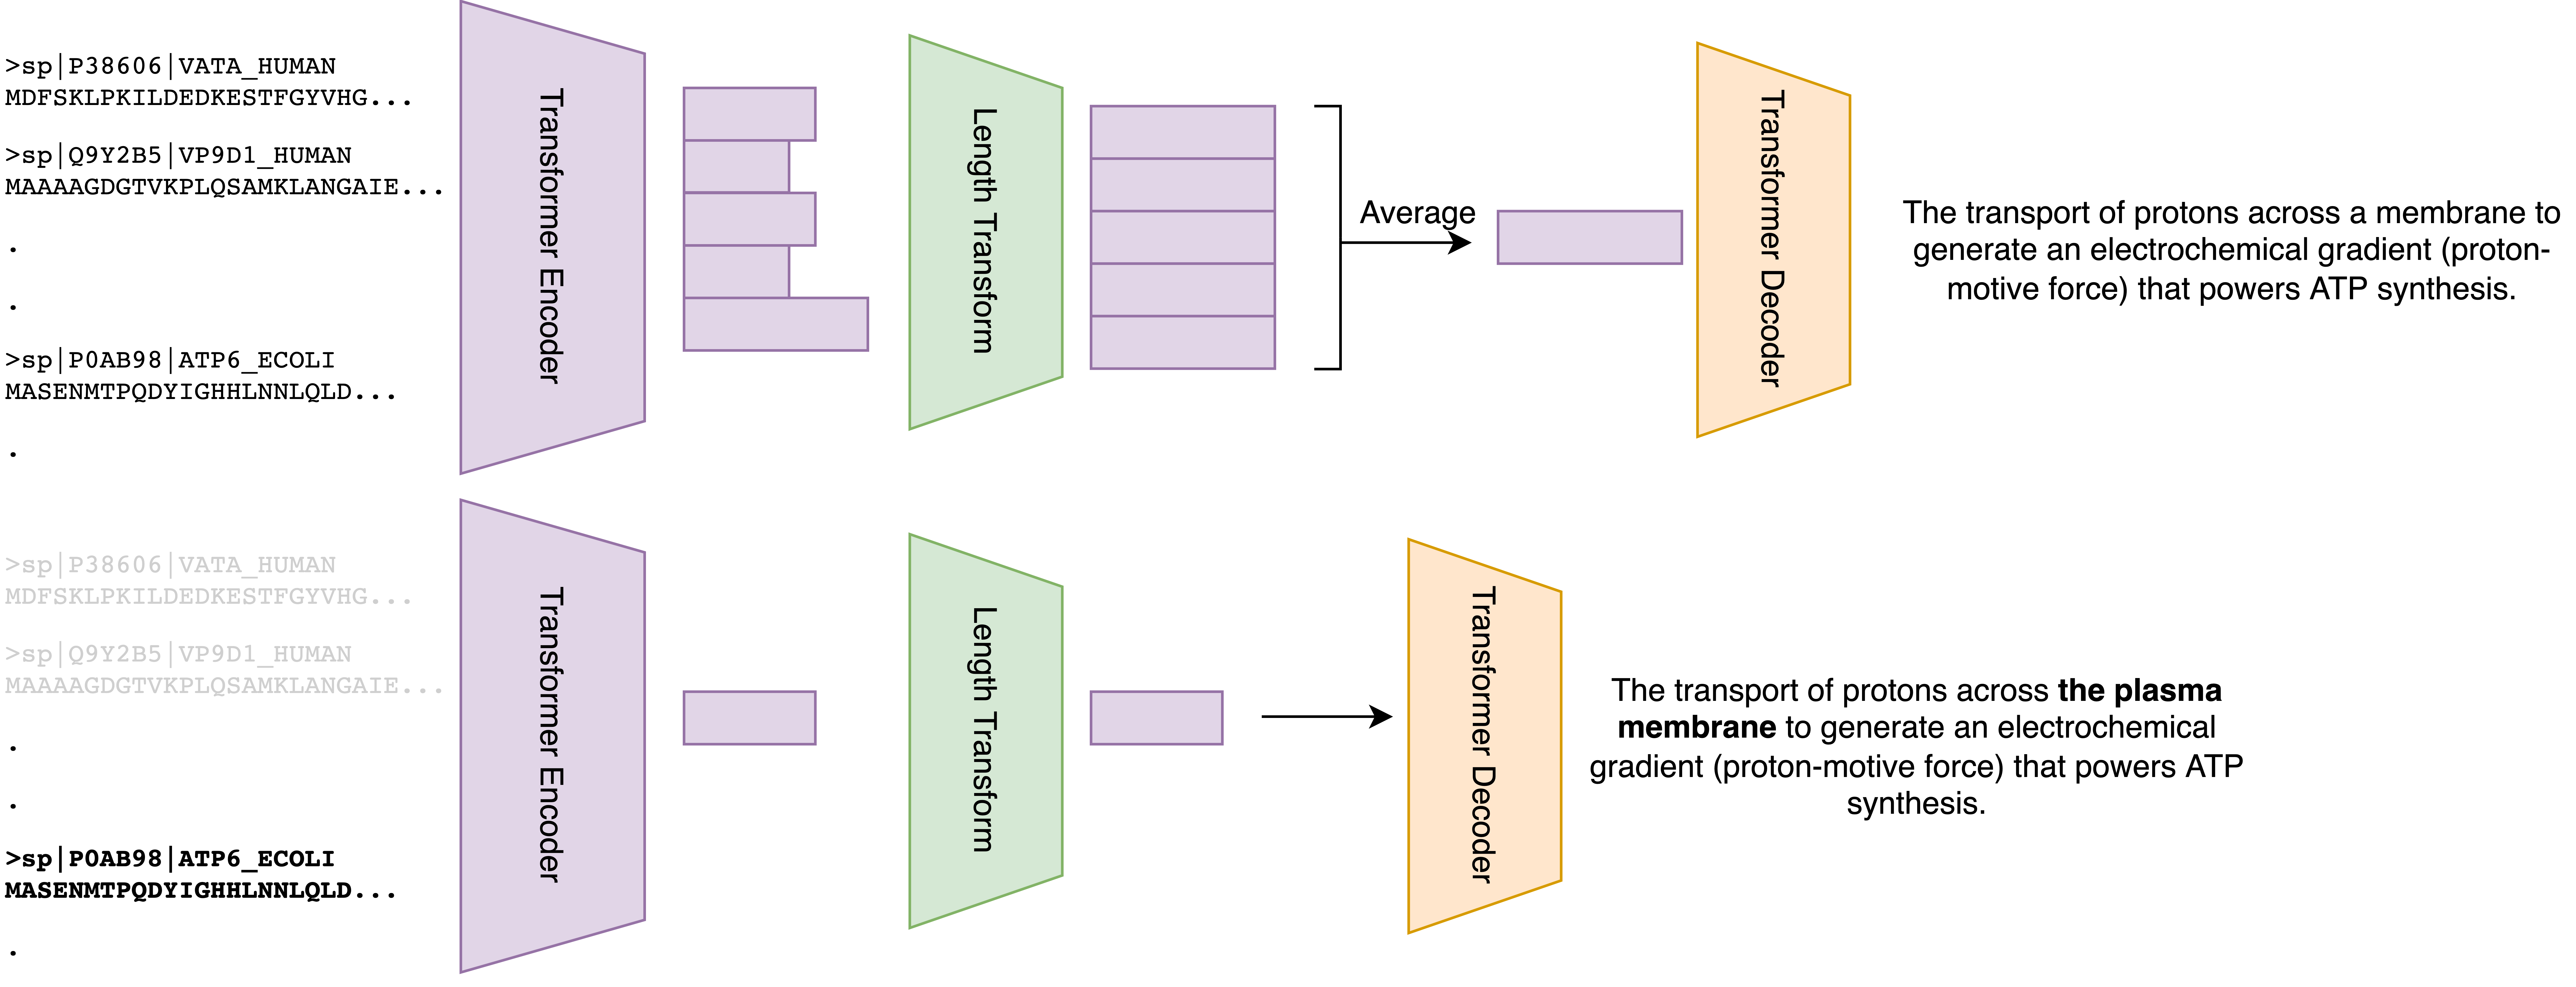
\includegraphics[width=0.9\linewidth]{prot2go.png}
    \caption{High-level diagram of the proposed transformer encoder-decoder model.
The model is trained to produce the most specific common function of the input protein sequences.}
    \label{overview}
\end{figure}

\begin{table}
	\caption{Sample Test Set Description Generations}
	\centering
    \begin{tabular}{p{8 cm}|p{8 cm}}
		\toprule
        True Common GO Description of Sequence Set & Model Generated Description of Sequence Set \\
		\midrule
        <SOS> the process in which the anatomical structures of appendages are generated and organized . an appendage is an organ or part that is attached to the trunk of an organism . <EOS> & <SOS> the process whose specific outcome is the progression of the eye over time , from its formation to the mature structure . <EOS> \\ \hline
        <SOS> any process that activates or increases the frequency , rate or extent of cell differentiation . <EOS> & <SOS> any process that modulates the frequency , rate or extent of cell differentiation . <EOS> \\ \hline
		<SOS> a protein complex that contains the gins complex , cdc45p , and the heterohexameric mcm complex , and that is involved in unwinding dna during replication . <EOS> & <SOS> any process involved in forming the mature 3 ' end of a dna ( mrna ) molecule . <EOS> \\
        \hline
        <SOS> the targeting and directed movement of proteins into a cell or organelle . not all import involves an initial targeting event . <EOS> & <SOS> the directed movement of proteins from endoplasmic reticulum to the nucleus . <EOS>  \\
		\bottomrule
	\end{tabular}
\end{table}

\begin{table}
	\caption{Model Performances. Correctness: The average number of times a correct GO term outranks an incorrect one for a given sequence set prediction. Specificity: Among correct GO terms, the average number of times a child outranks its parent. Robustness: The average rank correlation between the predictions of a pair of different identically annotated sequence sets.}
	\centering
	\begin{tabular}{l|l}
		\toprule
        Metric & Test set performance \\
		\midrule
        Annotation Correctness &  0.72 \\
        Specificity Preference &  0.58 \\
		Annotation Robustness &  0.26 \\
		\bottomrule
	\end{tabular}
	\label{tab:table}
\end{table}


\end{document}
